\chapter{Thresholding, Erosion, and Dilation}
\label{ch:lesson03}

Thresholding converts a grayscale image into a binary (black/white) image by comparing each pixel to a cutoff value. The result is often noisy, so it is cleaned up with two basic morphological operations: \textbf{erosion} (shrinks white regions, removes small specks) and \textbf{dilation} (grows white regions, fills small holes).

\section{Thresholding}

Thresholding is a per-pixel comparison: every pixel above the cutoff becomes white (255), every pixel at or below it becomes black (0). Figure~\ref{fig:l03-1} shows the noisy test image used throughout this chapter, and Figure~\ref{fig:l03-2} the result of thresholding it.

\begin{lstlisting}
binary = (noisy > threshold_value) * np.uint8(255)
\end{lstlisting}

\begin{figure}[h]
\centering
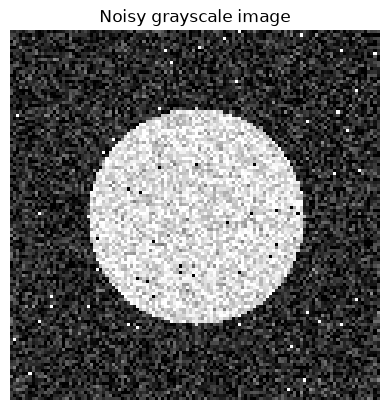
\includegraphics[width=0.35\textwidth]{figures/lesson03_fig01.png}
\caption{A synthetic bright circle on a dark background, with added noise and salt-and-pepper specks.}
\label{fig:l03-1}
\end{figure}

\begin{figure}[h]
\centering
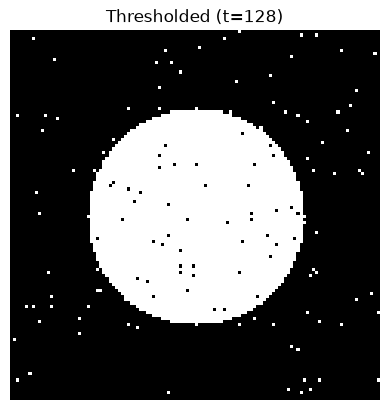
\includegraphics[width=0.35\textwidth]{figures/lesson03_fig02.png}
\caption{Simple thresholding at $t=128$.}
\label{fig:l03-2}
\end{figure}

OpenCV bundles the same operation into \code{cv2.threshold}, which for plain binary thresholding computes exactly the same result, and additionally supports variants such as inverted output, capping instead of zeroing, and automatic cutoff selection through the same function.

\subsection*{Otsu's method: choosing the threshold automatically}

The threshold above was picked by hand. \textbf{Otsu's method} (\citelink{otsu1979}{Otsu, 1979}) picks it automatically: it treats the image's histogram as a mixture of two classes (foreground and background) and searches over every possible cutoff for the one that minimizes the \emph{within-class} variance (equivalently, maximizes the variance \emph{between} the two classes).

\begin{lstlisting}
thresh_otsu, binary_otsu = cv2.threshold(
    noisy, 0, 255, cv2.THRESH_BINARY + cv2.THRESH_OTSU)
\end{lstlisting}

Figure~\ref{fig:l03-3} shows the resulting histogram and cutoff.

\begin{figure}[h]
\centering
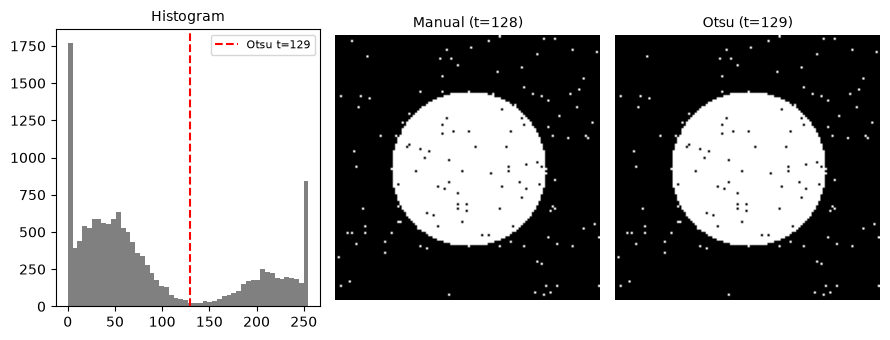
\includegraphics[width=0.95\textwidth]{figures/lesson03_fig03.png}
\caption{Histogram with the Otsu-selected cutoff, compared against the hand-picked threshold; the two results are visually near-identical here.}
\label{fig:l03-3}
\end{figure}

Otsu is a good default choice whenever a threshold is needed, but it will not work well with badly-separated or multi-modal histograms.

\section{Erosion and dilation}

There are two basic \textbf{morphological operations} for cleaning up the salt-and-pepper specks and ragged edges above.

\textbf{Erosion} slides a small \textbf{structuring element} (kernel) over the image; a pixel stays white only if the \emph{entire} kernel fits inside the white region, shrinking white regions and removing small specks. \textbf{Dilation} does the opposite: a pixel becomes white if the kernel overlaps \emph{any} part of the white region, growing white regions and filling small black holes.

\begin{lstlisting}
kernel = np.ones((3, 3), np.uint8)
eroded  = cv2.erode(binary, kernel, iterations=1)
dilated = cv2.dilate(binary, kernel, iterations=1)
\end{lstlisting}

Applying erosion then dilation --- an \textbf{opening} --- removes small white specks while restoring the size of the main region, a common way to denoise a thresholded image: \code{cv2.morphologyEx(binary, cv2.MORPH\_OPEN, kernel)}. Figure~\ref{fig:l03-4} compares all four results.

\begin{figure}[h]
\centering
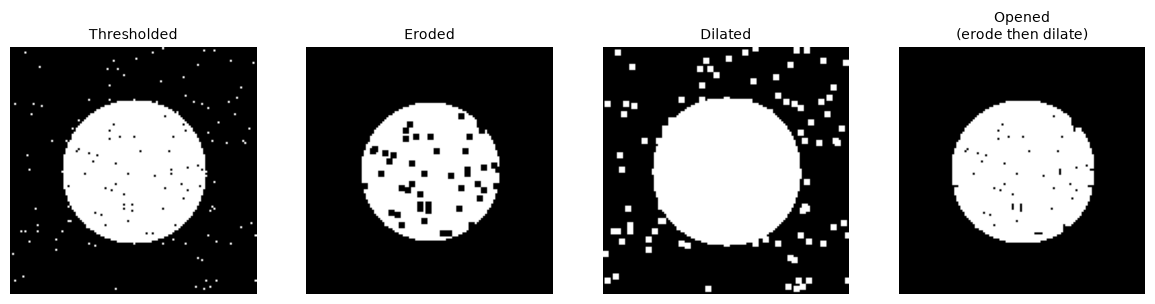
\includegraphics[width=0.95\textwidth]{figures/lesson03_fig06.png}
\caption{Thresholded, eroded, dilated, and opened (erode then dilate) versions of the same binary image.}
\label{fig:l03-4}
\end{figure}

\subsection*{Exercises}
\begin{enumerate}
  \item Try \code{cv2.MORPH\_CLOSE} (dilation followed by erosion) instead of \code{MORPH\_OPEN}. How does it differ, and which black-pixel noise does it fix that opening does not?
  \item Increase the kernel size to $(5,5)$. How does that change the result compared to $(3,3)$?
\end{enumerate}

\vfill
\fullcode{lesson03}{lesson03_thresholding_morphology}
